\section{User interface} \label{sec:user_interface}
In this section an analyzation of the user interface for the equalizer analyzed in \autoref{sec:tech_equalizer} will be made to determine which user interface will be the most optimal for the specific user of the equalizer. 

There are two different intended users for the equalizer: 
\begin{itemize}
\item The developer.
\item The commercial user.
\end{itemize}
This means that there are different requirements for the specific user of the equalizer.

\subsection{User interface for the developer}
The developer is the user which knows everything about an equalizer and its effects on a system therefore the developer desires a great deal of control and options in the interface of the equalizer. This means that the interface can be complex and must not set no restrictions for the developer.  

Because the developer needs to have full control of the equalizer he needs to have control of: 
\begin{itemize}
\item Center frequency.
\item Q - value.
\item Gain.
\item Band selection.
\end{itemize} 
This leads to a suggestions for a user interface which gives full control to a developer.

\begin{figure}[H]
\centering
\tikzsetnextfilename{InterfaceDev1}
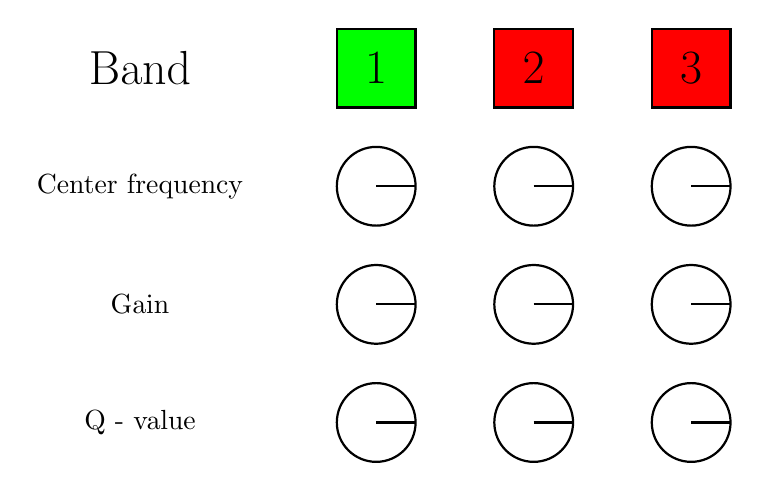
\begin{tikzpicture}
\draw[thick] (2,0) circle [radius=0.5] node at (-1,-0) {Q - value};
\draw[thick] (2,1.5) circle [radius=0.5] node at (-1,1.5) {Gain};
\draw[thick] (2,3) circle [radius=0.5] node at (-1,3) {Center frequency};
\draw node at (-1,4.5)[font=\LARGE]{Band};
\draw[thick][fill=green, draw=black](1.5,4) rectangle(2.5,5) node at (2,4.5)[font=\LARGE]{1};

\draw[thick] (4,0) circle [radius=0.5];
\draw[thick] (4,1.5) circle [radius=0.5];
\draw[thick] (4,3) circle [radius=0.5];
\draw[thick][fill=red, draw=black](1.5+2,4) rectangle(2.5+2,5) node at (2+2,4.5)[font=\LARGE]{2};

\draw[thick] (6,0) circle [radius=0.5];
\draw[thick] (6,1.5) circle [radius=0.5];
\draw[thick] (6,3) circle [radius=0.5];
\draw[thick][fill=red, draw=black](1.5+4,4) rectangle(2.5+4,5) node at (2+4,4.5)[font=\LARGE]{3};

\draw[thick](6,0) -- (6.5,0);
\draw[thick](6,1.5) -- (6.5,1.5);
\draw[thick](6,3) -- (6.5,3);

\draw[thick](4,0) -- (4.5,0);
\draw[thick](4,1.5) -- (4.5,1.5);
\draw[thick](4,3) -- (4.5,3);

\draw[thick](2,0) -- (2.5,0);
\draw[thick](2,1.5) -- (2.5,1.5);
\draw[thick](2,3) -- (2.5,3);
\end{tikzpicture}
\caption{Developer user interface.}
\label{fig:Dev_sug}
\end{figure}

The suggestion on \autoref{fig:Dev_sug} has push buttons on the bands so they can be toggled on and of while the center frequency, gain and Q - value for each band can be changed with the use of knobs. The suggestion will be accompanied by a big screen where the frequency response of the equalizer can be seen. 

\subsection{User interface for the commercial user}
The commercial user is the user which knows the implication of different the different settings of an equalizer but does not know anything about the technical aspect of an equalizer. This means that the interface needs to be simple and show what implpication a setting has on a system but leave out all technical aspects. 

Because the commercial user only needs presets like for example "rock", "jazz" and "movie" the user only needs to have control of: 
\begin{itemize}
\item Presets.
\end{itemize} 
This leads to some different suggestions for a user interface which consist of a few buttons to keep it as simple as possible.


\begin{figure}[H]
\centering
\begin{subfigure}[t]{0.47\textwidth}
	\centering
	\tikzsetnextfilename{InterfaceUser1}
	\scalebox{0.2}{

\begin{tikzpicture}
\draw [thick](-10,6) circle [radius=3];
\draw [thick](11,6) circle [radius=3];
\draw [thick](-6,4) -- (7,4) -- (7,8) -- (-6,8) -- (-6,4);
\draw[fill] (-12,6) -- (-10,8) -- (-9,8) -- (-11,6) -- (-9,4) -- (-10,4) -- (-12,6);
\draw[fill](13,6) -- (11,8) -- (10,8) -- (12,6) -- (10,4) -- (11,4)--(13,6) ;
\node[scale=8.0] (c) at (0.5,6) {Presets};
\end{tikzpicture}}
	\caption{Suggestion 1}
	\label{fig:UI_sug_1}
\end{subfigure}
\hspace{6mm} 
\begin{subfigure}[t]{0.47\textwidth}
	\centering
	\tikzsetnextfilename{InterfaceUser2}
	\scalebox{0.6}{
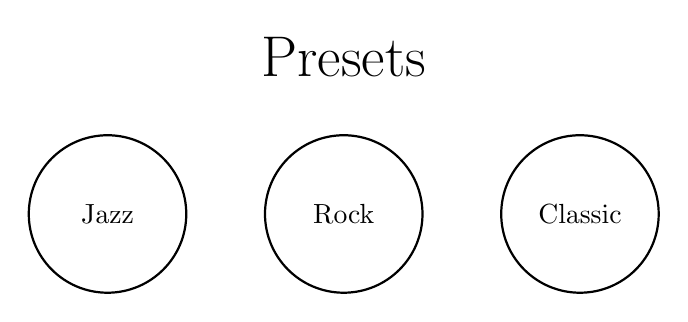
\begin{tikzpicture}
\draw [thick](0,0) circle [radius=1] node{Jazz};
\draw [thick](3,0) circle [radius=1] node{Rock};
\draw [thick](6,0) circle [radius=1] node{Classic};
\draw node at (3,2)[font=\huge]{Presets};
\end{tikzpicture}}
	\caption{Suggestion 2}
	\label{fig:UI_sug_2}
\end{subfigure}
\caption{Commercial user interface suggestions.}
\label{fig:UI_sug}
\end{figure}

Suggestion one as seen on \autoref{fig:UI_sug_1} has two push buttons and a small screen so the user can interchange between different settings, while suggestion two has x number of push buttons which represents a preset each. The advantage of suggestion two is the overview and simplicity while suggestion one can have a larger number of presets without changing the appearance of the user interface. 

The suggestions for the user interface for both the developer and the commercial user will be choosen in the requirement specification \todo[inline]{reference}  

